\chap{Enhanced Generative Adversarial Network}

\section{Introduction}

\section{GAN Architecture} 

The original paper's\cite{Original-GAN} generator architecture consisted of  rectifier linear\cite{RELU} and sigmoid activations, while the discriminator net used maxout [10] activations. the results were good but lacked stability and also suffered from the problem of model collapse.
Later, Radford \textit{et al.}\cite{DCGAN} proposed deep convolution generative adversarial network which used deep convolution with fractional stride convolution and batch normalization to stabilize the model. This work uses this architecture as base and later adding conditional vector to it. The figure 4.1 shows the architecture of generator and discriminator. In this work, we use RELU
in all the layers expect the output. Since the paper Radford \textit{et al.}\cite{DCGAN} showed that these can help in convergence of the model and it also covers the color space of the distribution.
\par

As you can see it figure the architecture of generator and discriminatory are exactly opposite to each other. The generator uses up-convolution or commonly known as backward convolution to generate image.%J. Long, E. Shelhamer, and T. Darrell, “Fully convolutional networks for semantic segmentation,”CoRR, vol. abs/1411.4038, 2014. [Online]. Available: http://arxiv.org/abs/1411.4038
The discriminator is a standard deep convolution neural network used for classification of real or  a fake image.
\begin{figure}
  \centering
    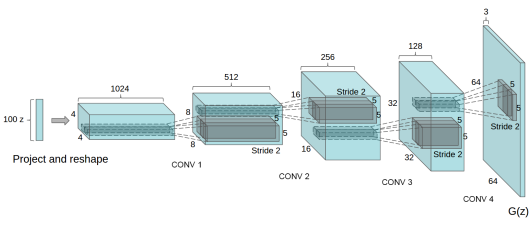
\includegraphics[scale=.7, angle=0]{Files/Generator-Architecture.png}
    \caption[Generator Architecture]{Generator Architecture\cite{DCGAN}}
    \label{fig: DCGAN}
\end{figure}

\section{Training GAN}

Training a GAN is always a tricky part. This work uses DCGAN\cite{DCGAN} as baseline, as the DCGAN has shown that it can stabilizes the networks to a great extent. The major contribution of the DCGAN in our work is the use of Batch-Normalization, strided convolution and ADAM optimizer. We will go through each of these steps one by one.
\subsection{BatchNomalization}

Batch Normalization was first introduced by Ioffe \textit{et al.}\cite{BatchNorm}. It is a major landmark in area of deep learning as most of the current deep neural network frameworks contains batch normalization. 
To understand batch normalization, we need to understand the problem it is trying to solve. Its major aim is to minimize internal co-variance shift. Internal covariance shift refers to the change in input distribution as we are feeding data in mini batches. Since a neural network are designed in hierarchical fashion, so even small change in form of an outlier can get amplified as we are dealing with generally more than a million parameters and several layers. To rectify this problem, we normalize each batch at every layer, by both mean and variance. This process is commonly called as whitning. The major advantages of the batch normalization are as follows.
\begin{itemize}
    \item Initial value of weights have less impact on gradient descent.
    \item It helps in keeping higher learning rate and accuracy. Hence it reduces overall training time and this helps in faster training of the GANs.
\end{itemize}

\subsection{Strided Convolution}

The concept of deconvolution was first introduced by Zeiler \textit{et al} \cite{Deconv}. It also is commonly known as  strided convolution, transposed fractional convolution or upsampling.



\par
It basically is going from output of some convolution to the input to that convolution.For instance it is going from green matrix to the blue matrix as shown in below figure. So given a kernel K, the type of convoution is defined by how forward or backward passes are calculated\cite{Deconv-Theano}.


\begin{figure}[ht]
  \centering
    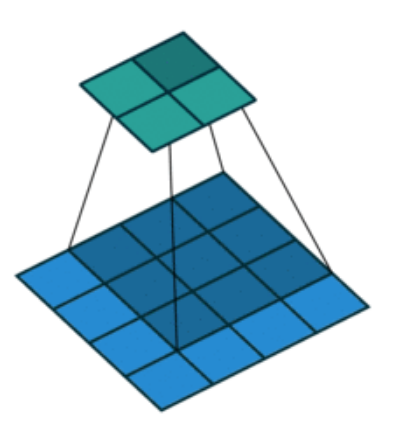
\includegraphics[scale=.5, angle=0]{Files/simple-conv.png}
    \caption[Simple Convolution]{Simple Convolution \cite{Deconv-Theano}}
    \label{fig: Simple Convolution}
\end{figure}

\begin{figure}[ht]
  \centering
    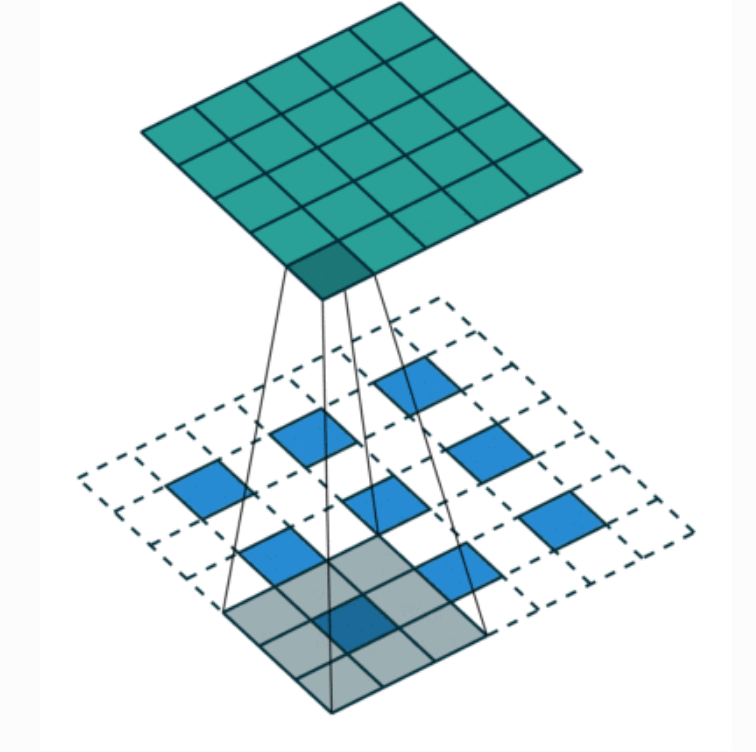
\includegraphics[scale=.4, angle=0]{Files/Frational-Stride-Conv.png}
    \caption[Transpose Convolution ]{Transpose Convolution \cite{Deconv-Theano}}
    \label{fig: Strided Convolution}
\end{figure}



\subsection{ADAM Optimizer}

Adaptive Moment Estimation whihc more commontly known as ADAM optimizer is a stochastic gradient descent(SGD) optimizer. It was first proposed by Diederik \textit{et al.} \cite{Adam}. The vanilla stochastic gradient descent suffers from many problems. But the three key issues which directly related to our work are as follows.
\begin{itemize}
    \item In case of non convex error function, the neural network can be stuck at non local optima.
    \item Choosing correct learning is always a challenging task and it can cause longer time for SGD algorithm to converge.
    \item Specifically in our work, where we are trying to model the data and it is sparse. Vanilla SGD doesn't provide flexibility for having different learning rate for each weight.

To overcome this problem we use ADAM optimizer in our work. It combines adagrade\cite{Adagrade} and momentum-optimizer \cite{momentum}. It 

\end{itemize}
 
 
 